\chapter{Quantifying dynamism in compiler framework pattern rewriting}
\label{chap:dynamism-pattern-rewriting}

%% Introduction
% Hook
A key difference between the Python and C++ runtimes is their degree of dynamism.
% Argument
\ac{mlir}'s C++ runtime incurs overhead when dynamically dispatching functions (\autoref{fig:narrative}, \circledbase{pairedThreeLightGreen}{3}), which is worsened by prohibiting ahead-of-time performance optimisations. In contrast, almost every bytecode operation evaluated by the Python interpreter is dynamic, each incurring an overhead.
As such, we expect the difference in performance between language runtimes (\autoref{fig:narrative}, \circledbase{pairedFourDarkGreen}{4}) to be smaller for more dynamic workloads.
% Link
In this chapter, we quantify this difference by examining simple examples within static and dynamic language runtimes. We then apply this information to understand the difference in performance between pattern rewriting workloads using xDSL and \ac{mlir} through the lens of overhead incurred by dynamism.


% \section{Quantifying the performance cost of dynamism in static languages}
% % Hook
% Having specialised our micro-benchmarks of xDSL to the most minimal implementation which expresses the desired functionality (\autoref{chap:specialising-optimising-pattern-rewriting}), we can use them to draw comparisons between equivalent \ac{mlir} benchmarks. This allows us to minimise the impact of implementation details, instead measuring the effect of the language runtime on each framework's performance.
% % Argument
% Of these micro-benchmarks, operation trait checking is particularly suitable for detailed analysis. This is because both implementations (Listing \ref{listing:ubenchmark-trait-checks-both}) share the same underlying algorithm: iteration over an operations traits, checking the \ac{rtti} of each one.
% % Link
% We discuss two notable sources of performance overhead incurred by dynamism in this workload: dynamically dispatching function calls; and checking \ac{rtti} of polymorphic objects. % + object access



\subsection{Run-time type information}

%% Introduce the issue
% Hook
In a ``A history of C++: 1979--1991'', Stroustop states that in the original C++ design he ``deliberately didn't include [mechanisms] for run-time type identification [as] they were almost always misused.'' \cite{stroustrupHistory197919911996}.
% Argument
Support for this functionality was later added in C++98 \cite{internationalorganizationforstandardizationISOIEC148821998}, adding support for \texttt{dynamic\_cast}s checked a runtime, and getting the \texttt{typeid} of a polymorphic object. LLVM reimplements a subset of this functionality, providing the \texttt{dyn\_cast} method and \texttt{TypeID} data structure, aiming to ``strike a balance between performance and the setup required to enable its use'' \cite{mlirteamMLIRCodeDocumentation}.
This is another example of dynamic behaviour, which we again argue incurs additional runtime overhead and precludes optimisations in static languages, closing the gap with dynamic ones.
% Link
As before, we justify this be examining the details of this mechanism, using both synthetic examples and our micro-benchmark suite.

%% Experiment setup
%% Discussion of these results (single number on overhead)

%% Graph
% If known at runtime -> zero cost + revealed optimisations (cannot easily quantify!)
% dyn_cast
% dynamic_cast
% isinstance
\begin{figure}[H]
    \centering
    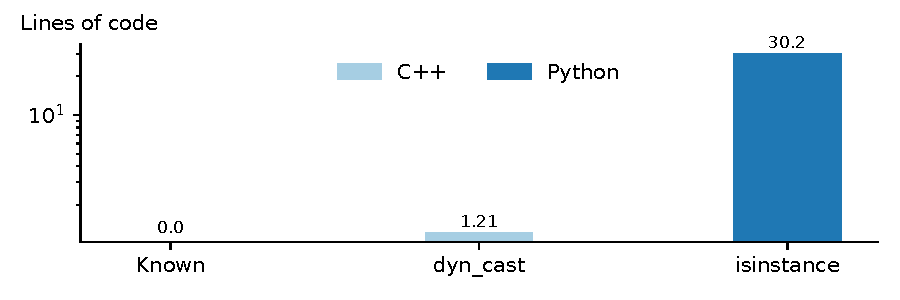
\includegraphics[width=0.75\textwidth]{images/impact_dynamism/dynamic_cast.pdf}
    \caption{.}
    \label{figure:impact-rtti}
\end{figure}




% %% Where is the issue in the micro-benchmark?
% % Hook
% By leveraging Python's dynamic nature, xDSL can invoke the \mintinline{python}{isinstance} function to check the type information each trait. In contrast, \ac{mlir} uses template meta-programming instead of the class hierarchy to define traits. This depends on \mintinline{c++}{TypeID}\footnote{\scriptsize{\url{https://mlir.llvm.org/doxygen/TypeID_8h_source.html}}}, a custom data structure to encode dynamic \ac{rtti} in C++. This is performant, as the \mintinline{c++}{TypeID} data structure is constructed to remedy many of the issues of native C++ \ac{rtti}.
% % Argument
% % Link






\subsection{Cost of dynamic dispatch}

%% Introduce the issue, and where it is in the micro-benchmark
% Hook
In static languages such as C++, the exact address of many function calls can be resolved at compile time. In contrast, dynamic languages such as Python must resolve the address of each function call at runtime, incurring an overhead.
% Also optimisation boundary and stuff
% Argument
However, the address of some function calls can only be known at runtime, for example as a result of object polymorphism. This address then must be resolved during execution by the language runtime in both static and dynamic languages. Furthermore, this information being known only at runtime presents and optimisation boundary, precluding common rewrites such as function inlining which contribute to the performance of ahead-of-time compiled languages.
As such, we argue there the difference between static and dynamic languages is reduced for highly dynamic workloads with insufficient information to resolve function addresses ahead of time.
% Link
We justify this by examining the mechanisms of dynamic dispatch in Python and C++, and contrasting them through both synthetic examples and our micro-benchmark suite.

%% How do vtables work and CPython stuff work
% Hook
For the common example of method polymorphism, C++ uses a \ac{vtable} to support dynamic dispatch.
% Argument
When a virtual function is called on an object, the compiler resolves the address of that function by following an associated pointer to its \ac{vtable}. It then indexes into this data structure to retrieve the function address, which it can then execute. This indirection allows runtime information to be used to resolve the function address, but incurs a small overhead of a pointer dereference.
In Python, this indirection is present irrespective of whether the function address could be inferred ahead of time. Python objects have a \mintinline{text}{__dict__} mapping storing both their methods and attributes. Similarly to the \ac{vtable}, this is indexed to retrieve the function address at runtime. If the name is not found, the interpreter checks the mapping for each of its parents in the inheritance hierarchy according to its method resolution order. This approach supports dynamic behaviour such as runtime meta-programming, but incurs a higher performance cost than C++.
% Link
We can quantify the performance overhead of this \ac{vtable} mechanism through a synthetic example.

% %% Quantifying with toy example, and how to count in real-world
% % Hook
% This shows that...
% % Argument
% The pointer dereference cost is small. The hidden optimisation opportunities are bigger. Python is much slower, and a two-step process (LOAD\_METHOD + CALL\_METHOD), where LOAD\_METHOD is slow.

%% TODO: Shout this out better?
% Hook
In addition to quantifying the performance of \ac{vtable} accesses, we can also estimate the number of dynamic calls made for a running workload.
% Argument
In the ARM instruction set, direct and indirect calls \cite{armlimitedARMCortexRSeries}
``Because the branch destination is PC-relative, it can be determined exactly at an early stage of the pipeline''. This means that direct calls are more performant, and as such efficient compilers only use indirect calls where address information is not known ahead of time: dynamic control flow.
Using the \texttt{perf} tool, we can leverage hardware performance counters to total the number of indirect calls made.
% Link

% %% Where does this occur?
% % Hook
% This behaviour
% % Argument
% % Link
% In other cases, \ac{mlir} is implemented to avoid this overhead. For example, the \mintinline{text}{TypeID::get<Traits>} function uses template meta-programming to monomorphise the generic function calls. However, this approach is only applicable when there is sufficient information at runtime.

% \subsection{Object data access}
% __slots__ and polymorphism stuff

\subsection{Hiding ahead of time optimisations}








% \section{Dynamism in pattern rewriting}

%% Introduction

%% Something about RTTI
%% Count up vtable invocations in C++ to argue about dynamic dispatch

%% Estimate lower bound for cost of dynamism

%% Summary
